\documentclass[11pt,a4paper]{article}

\usepackage[provide=*,spanish]{babel}
\usepackage[utf8]{inputenc}
\usepackage[T1]{fontenc}
\usepackage{lmodern}
\usepackage[margin=2.35cm]{geometry}
\usepackage{amsmath}
\usepackage{booktabs}
\usepackage{tabularx}
\usepackage{array}
\usepackage{enumitem}
\usepackage{xcolor}
\usepackage{microtype}
\usepackage{parskip}
\usepackage{titlesec}
\usepackage{hyperref}
\usepackage{graphicx}
\usepackage{caption}
\usepackage{float}

\definecolor{azulWCD}{RGB}{17,67,112}
\definecolor{azulClaro}{RGB}{232,241,249}
\definecolor{rojoAviso}{RGB}{160,40,30}

\hypersetup{
  colorlinks=true,
  linkcolor=azulWCD,
  urlcolor=azulWCD,
  pdftitle={Flujo de neutrones sobre Bucaramanga: revision de las secciones 4.3 a 4.5},
  pdfauthor={Jaime A. Betancourt}
}

\titleformat{\section}{\normalfont\Large\bfseries\color{azulWCD}}{\thesection}{0.6em}{}
\titleformat{\subsection}{\normalfont\large\bfseries\color{azulWCD}}{\thesubsection}{0.6em}{}

\newcommand{\ok}{\textcolor{green!50!black}{\textbf{OK}}}
\newcommand{\alerta}{\textcolor{rojoAviso}{\textbf{Revisar}}}
\newcommand{\nota}{\textcolor{orange!80!black}{\textbf{Nota}}}
\newcommand{\archivo}[1]{\texttt{\detokenize{#1}}}

\title{\color{azulWCD}\textbf{Flujo de neutrones sobre Bucaramanga (956 m s.n.m.)}\\[0.3em]
\large Revisión técnica de las secciones 4.3, 4.4 y 4.5 de la tesis}
\author{Jaime A. Betancourt}
\date{27 de septiembre de 2026}

\begin{document}
\maketitle

\begin{abstract}
Se revisan las secciones 4.3 (campo de neutrones atmosféricos sobre la superficie de
Bucaramanga), 4.4 (respuesta del WCD al flujo atmosférico rápido y de alta energía) y 4.5
(respuesta del WCD al flujo emergente de un suelo seco) de la tesis \emph{Evaluación mediante
simulación Monte Carlo de un detector Cherenkov de agua dopado con NaCl para la medición de
neutrones cósmicos con aplicación en monitoreo de humedad del suelo en Colombia} (páginas
222--251 de la numeración impresa; 248--277 del PDF). Para cada subsección se resumen sus
características y se contrastan las cifras con los archivos de partículas y los notebooks que
las generaron. La mayoría de las cifras se reproducen exactamente. Se identifican dos problemas
de fondo: (i) el conjunto ``rápido'' de la sección 4.4 es el archivo ARTI de 3600~s y está
normalizado a 12~h, y además empieza en 20~MeV y no en 1~MeV; (ii) el tiempo de exposición de
12~h del archivo completo no puede confirmarse a partir de los datos. Los notebooks
correspondientes se entregan junto a este informe en
\archivo{analysis/flujo-bucaramanga_secciones-4.3-4.5/}.
\end{abstract}

\section*{Archivos de partículas utilizados}

{\small
\begin{tabularx}{\textwidth}{>{\raggedright\arraybackslash}p{5.6cm} r >{\raggedright\arraybackslash}X}
\toprule
Archivo & Neutrones & Contenido verificado \\
\midrule
\archivo{flujo_neutrones_completo_Bga.shw}\newline (= \archivo{all_bga_neutron_35.shw}) & 1\,891\,124 &
Campo en superficie ARTI + suelo, $3.5\times10^{-11}$--$4.2\times10^{5}$~MeV; 1\,111\,010
descendentes y 780\,114 ascendentes (41~\%). Momentos en MeV/$c$, posiciones en un plano de
$400\times400$~m. \\
\archivo{flujo_neutrons_rapidos_Bga.shw}\newline (= \archivo{S3_bga_003600_neutrons_MeV.shw}) & 317\,537 &
Salida directa de ARTI, sólo neutrones descendentes con $E\ge 20.0009$~MeV. Idéntico línea a línea
al archivo ARTI \archivo{S3_bga_003600} (``003600'' = 3600~s). \\
\archivo{flujo_neutrones_suelo_seco_Bga.shw}\newline (= \archivo{filtered_neutrons.shw}) & 207\,969 &
Subconjunto del archivo completo: $10^{-8}$--$10^{-5}$~MeV y \emph{todos} ascendentes
($p_z>0$). La selección direccional que describe la tesis está confirmada. \\
\bottomrule
\end{tabularx}}

\section{Sección 4.3 --- Campo de neutrones atmosféricos sobre Bucaramanga}

\paragraph{Características del espectro (Fig.~4.52).}
Es el espectro por unidad de letargía $d\Phi/du$ de todo el archivo de superficie, con 300
intervalos logarítmicos (20 por década) entre $10^{-10}$ y $10^{5}$~MeV. La tesis lo describe
correctamente como la superposición del flujo atmosférico descendente y del albedo ascendente
(Ec.~4.39). Recalculadas con el CSV del notebook, sus características son las siguientes:

\begin{table}[H]
\centering\small
\begin{tabular}{l l r r}
\toprule
Población & Intervalo & Fracción de neutrones & Máximo de $d\Phi/du$ \\
\midrule
Térmica          & $<10^{-7}$ MeV ($<0.1$ eV)        & 9.5~\%  & $4.2\times10^{-8}$ MeV (0.042 eV) \\
Epitérmica       & $10^{-7}$--$10^{-6}$ MeV          & 4.1~\%  & --- \\
Intermedia       & $10^{-6}$--$10^{-1}$ MeV          & 21.7~\% & meseta \\
Evaporación      & $0.1$--$20$ MeV                   & 28.7~\% & 2.4 MeV \\
Cascada          & $>20$ MeV                         & 36.1~\% & 133 MeV \\
\bottomrule
\end{tabular}
\end{table}

Un ajuste maxwelliano a la región térmica da $kT=25.8\pm1.1$~meV ($T\simeq299$~K), lo que
confirma que el momento está en MeV/$c$.

\begin{figure}[H]
\centering
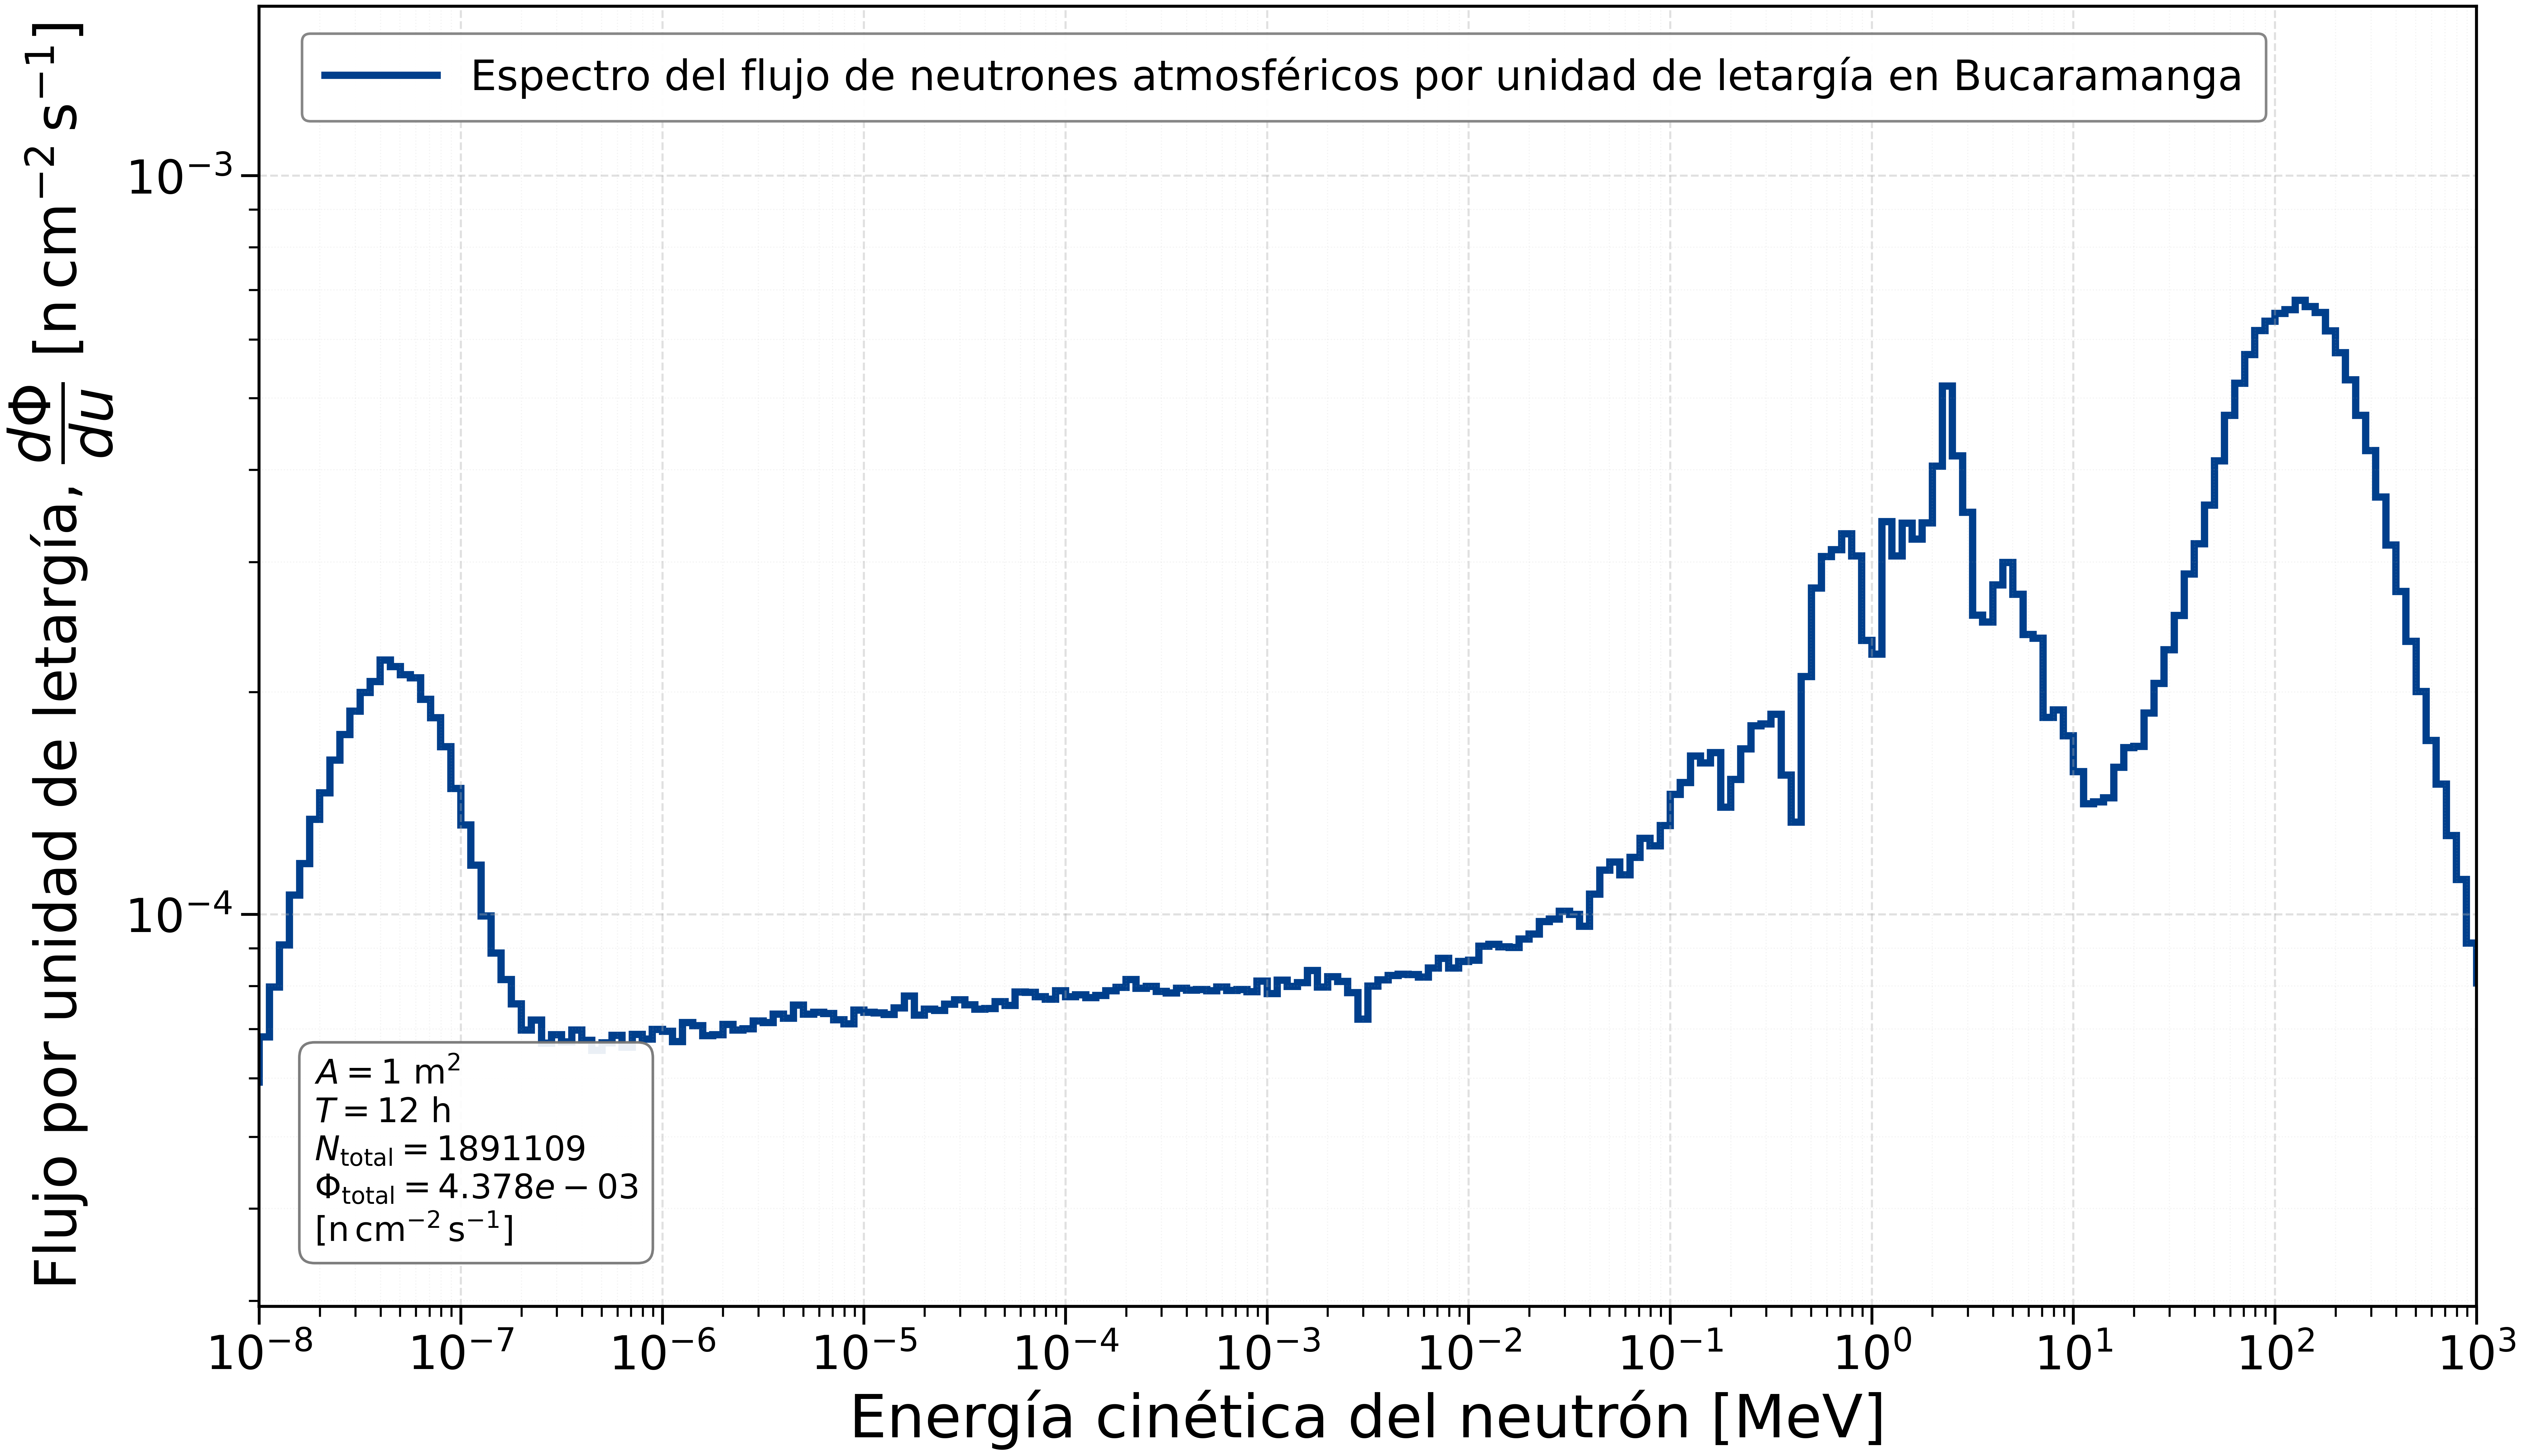
\includegraphics[width=0.72\textwidth]{figuras/Flujo-letargico-completo-Bucaramanga.png}
\caption{Figura 4.52 regenerada por \archivo{Flujos-neutrones-Bga.ipynb}.}
\end{figure}

\paragraph{4.3.1 Normalización temporal.}
$\Phi_n = N_n/(A\,t) = 1\,891\,109/(10^4\,\text{cm}^2 \times 43\,200\,\text{s}) =
4.378\times10^{-3}$~n\,cm$^{-2}$\,s$^{-1}$; $N_{1h}=1.576\times10^{5}$. La aritmética es
correcta (\ok). Hay tres observaciones:
\begin{enumerate}[leftmargin=*,itemsep=2pt]
\item \alerta\ \textbf{Las 12 h son un supuesto, no un dato.} Nada en el archivo lo fija.
  Además, el archivo completo contiene 647\,984 neutrones descendentes con $E>20$~MeV, sólo
  $2.04\times$ los 317\,537 del archivo ARTI de 3600~s (Fig.~\ref{fig:verif}b). Si el completo
  correspondiera a 12~h con la misma área y el mismo ARTI, el cociente sería $\approx12$.
  Tampoco es constante: crece de 2.0 a 4.3 con el umbral, así que ambos archivos no provienen
  de la misma corrida y no basta un simple reescalado temporal. Hay que documentar el parámetro
  \texttt{-t} de ARTI y el área efectiva con que se generó \archivo{all_bga_neutron_35}.
\item \nota\ El texto dice que el archivo completo ``contiene 1\,891\,109 historias; 1\,847\,307
  de ellas dentro del intervalo representado''. El archivo tiene \textbf{1\,891\,124}. Hay
  1\,891\,109 en $[10^{-10},10^{5}]$~MeV, que es el valor de la leyenda. La cifra 1\,847\,307
  no se reproduce con ningún corte natural: con $E\le10^{3}$~MeV da 1\,865\,575 y con
  $E\ge10^{-8}$~MeV da 1\,872\,841.
\item \nota\ $N/(A\,t)$ cuenta cruces del plano en ambos sentidos. Es una \emph{corriente}
  bidireccional, no el flujo escalar. El flujo escalar ($\sum 1/|\cos\theta|$) es
  $\approx1.62$ veces mayor para este archivo. Conviene nombrar la magnitud con precisión.
\end{enumerate}

\paragraph{4.3.2 Espectro diferencial y flujo integrado.}
La definición $(d\Phi/du)_i=N_i/(A\,t\,\Delta u_i)$ y la recuperación del total mediante
$\sum_i(d\Phi/du)_i\Delta u_i=\sum_i N_i/(A\,t)$ son correctas. El notebook obtiene el mismo
$4.377567\times10^{-3}$ por ambas vías (\ok). En la Ec.~4.62 aparecen comas espurias
(``$A,\,t$'').

\paragraph{4.3.3 Interpretación física.}
La lectura por regiones es cualitativamente correcta. Hay que precisar dos cosas. La
estructura térmica tiene su máximo en $\approx4\times10^{-8}$~MeV (0.04~eV, maxwelliana a
temperatura ambiente) y no en $10^{-8}$~MeV (0.01~eV). El ``pico rápido'' entre $10^{-1}$ y
$10^{1}$~MeV es la componente de evaporación (máximo en 2.4~MeV), que reúne el 28.7~\% de los
neutrones y no aparece en el conjunto de la sección 4.4.

\section{Sección 4.4 --- Flujo atmosférico rápido y de alta energía}

\begin{figure}[H]
\centering
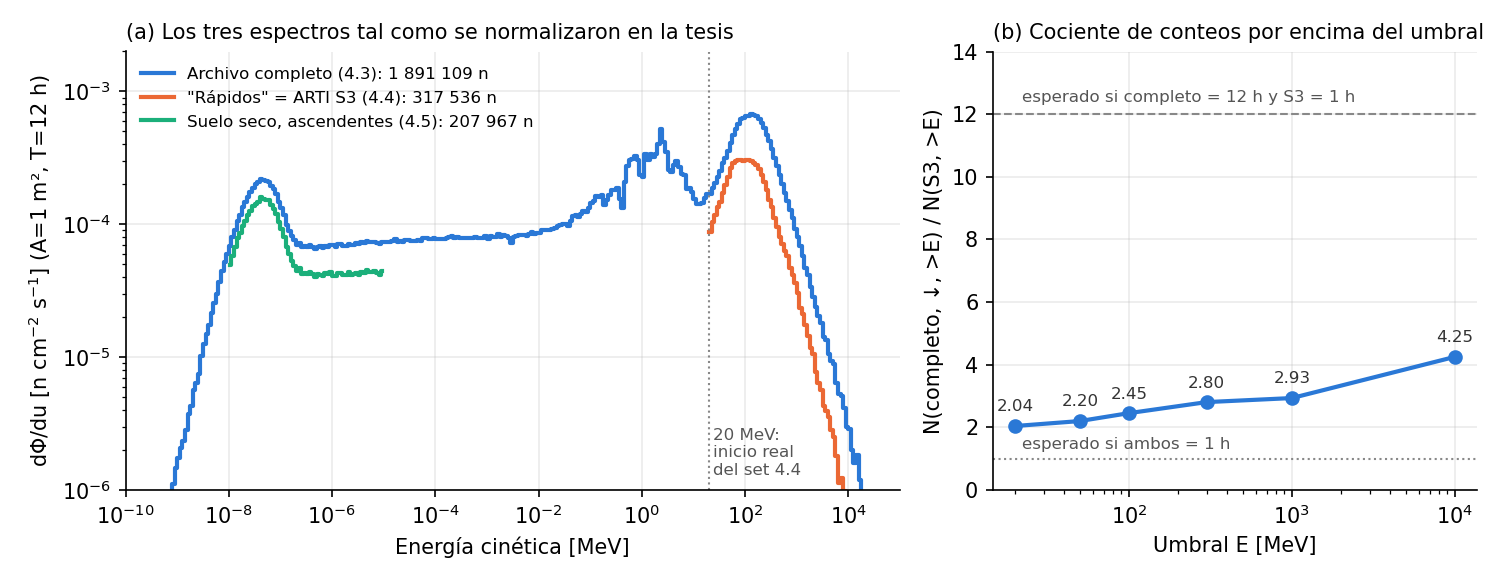
\includegraphics[width=\textwidth]{figuras/verificacion_normalizacion_temporal.png}
\caption{(a) Los tres espectros tal como aparecen en las Figs.~4.52, 4.53 y 4.61 (misma
normalización $A=1$~m$^2$, $T=12$~h). El conjunto de la Sec.~4.4 (naranja) empieza en 20~MeV.
(b) Cociente entre los neutrones descendentes del archivo completo y los del archivo ARTI de
3600~s por encima de cada umbral.}
\label{fig:verif}
\end{figure}

\paragraph{4.4.1 Intervalo de energía.}
\alerta\ La tesis declara $1\le E_k\le10^{5}$~MeV y afirma que el conjunto ``incluye una
fracción de la región de neutrones rápidos''. El archivo empieza en \textbf{20.0009~MeV} (el
corte de la salida de ARTI) y llega a $1.35\times10^{5}$~MeV (un neutrón queda fuera de la
figura). No hay ningún neutrón entre 1 y 20~MeV. El ``incremento del flujo a partir de
aproximadamente 20 MeV'' de la Fig.~4.53 es, por tanto, el borde de la selección y no una
característica física. El máximo de $d\Phi/du$ está en 75~MeV.

\paragraph{4.4.2 Normalización, número de neutrones y flujo integrado.}
$317\,536/(10^{4}\times43\,200)=7.350\times10^{-4}$~n\,cm$^{-2}$\,s$^{-1}$ es aritméticamente
correcto. Sin embargo, \alerta\ el archivo es la salida ARTI de \textbf{3600~s}. Si se normaliza
con su tiempo real, el flujo es $8.82\times10^{-3}$~n\,cm$^{-2}$\,s$^{-1}$ (88.2~n\,m$^{-2}$\,s$^{-1}$),
12 veces mayor que el valor de la tesis. Esto afecta a la Fig.~4.53, al texto de 4.4.2 y a
cualquier tasa por unidad de tiempo derivada de este conjunto.

\paragraph{4.4.3 Humedad del suelo y del aire.}
Es un argumento cualitativo y físicamente razonable: la componente $>20$~MeV es poco sensible
a la humedad y el vapor de agua pesa menos que el agua del suelo. No se apoya en ninguna
simulación con distintos contenidos de agua, así que debe presentarse como expectativa y no
como resultado.

\paragraph{4.4.4 Definición del flujo incidente.}
Es coherente: la cascada ($\sim10^{2}$~MeV) es la fuente que, tras moderarse, alimenta las
poblaciones de menor energía. \nota\ Falta indicar qué archivo y cuántas historias primarias se
inyectaron en el WCD para 4.4.5--4.4.9. Los datos de esas subsecciones se llaman
``\archivo{flujo-completo}'' y los de distancias llevan el sufijo ``\archivo{_1h}''. Además, a
diferencia de 4.5, no se reporta la fracción de captura sobre el número de incidentes.

\paragraph{4.4.5 Partículas secundarias (Figs.~4.54--4.55).}
Las líneas y los bordes Compton rotulados son correctos:
$E_C=2E_\gamma^2/(m_ec^2+2E_\gamma)$ da 1.99, 5.86 y 8.33~MeV para 2.223, 6.11 y 8.58~MeV (\ok).
La tendencia de crecimiento con NaCl coincide cualitativamente con Sidelnik y col.\ (2020), y
la tesis ya advierte con acierto que no se trata de una validación absoluta. Notebooks:
\archivo{Analisis-gamma.ipynb}, \archivo{Analisis-gamma-AP-Flujo-completo.ipynb} (Fig.~4.55) y
\archivo{Analisis-Espectro-Electrones.ipynb}.

\paragraph{4.4.6 Distribución espacial de capturas.}
Las conclusiones (simetría axial conservada, $\sigma_r\approx11$~cm casi independiente del
NaCl, capturas desplazadas hacia la entrada al aumentar la salinidad) son consistentes con las
figuras del Apéndice~F. La reformulación final de la tesis es la correcta: el NaCl cambia la
profundidad de captura, no el ancho radial. Errata: ``En en el Apéndice''.

\paragraph{4.4.7 Moderación (Figs.~4.57--4.58).}
La tabla de la Fig.~4.57 se reproduce exactamente a partir del archivo de resultados
($\langle N\rangle$ = 110.87, 85.78, 70.81, 53.80; $N_\text{capt}$ = 164\,723 a 175\,715)
(\ok). La interpretación prudente, que atribuye la reducción de $\langle N\rangle$ a la
selección de historias más cortas, es adecuada. Errores de edición: referencia rota
``Sección (4.23)'' y ``alta \emph{alergia}''. \nota\ El notebook del flujo completo no contiene
la celda que genera la Fig.~4.58 ($\langle\xi\rangle=0.159$--$0.322$). Sus celdas de $\xi$ leen
archivos \archivo{cita-*-termicos-Bga} del suelo seco, así que conviene identificar y conservar
el código fuente de esa figura.

\paragraph{4.4.8 Distancias de captura.}
El máximo está en 9.0--10.0~cm y la media en 15.8--16.6~cm, con $\sigma\approx11.4$~cm. Esto
es consistente con ``entre 5 y 15 cm'' (\ok). \nota\ Estas distribuciones tienen entre
139\,845 y 151\,084 eventos, frente a los 164\,723--175\,715 capturas de la Fig.~4.57. Son
selecciones distintas, probablemente sólo las capturas dentro del volumen activo, y conviene
declararlo.

\paragraph{4.4.9 Respuesta fotoelectrónica.}
La descripción de la Fig.~4.60 es cualitativa: agua pura domina en 0--15 fotones y el NaCl al
10~\% en 15--100. No se encontró en las carpetas revisadas el notebook que produce esa figura
de cuatro paneles. Hay que localizarlo y añadirlo a la carpeta.

\section{Sección 4.5 --- Flujo de neutrones emergentes de un suelo seco}

\paragraph{4.5.1 Intervalo de energía.}
$1.0001\times10^{-8}$--$1.00002\times10^{-5}$~MeV (0.01--10~eV) (\ok). Se confirma que los
207\,969 neutrones son ascendentes.

\paragraph{4.5.2 Características del flujo diferencial.}
El máximo está en $4.2\times10^{-8}$~MeV, dentro del intervalo $3$--$7\times10^{-8}$ citado
(\ok). La composición es 55.6~\% térmica, 23.9~\% epitérmica y 20.5~\% en 1--10~eV, lo que
coincide con la descripción ``dominado por térmicos''. La lectura de no-equilibrio (campo
abierto) es correcta.

\paragraph{4.5.3 Flujo integrado.}
$4.814\times10^{-4}$~n\,cm$^{-2}$\,s$^{-1}$ se reproduce (\ok). \alerta\ El texto afirma que el
eje de la Fig.~4.61 es $d\Phi/dE$ [n\,cm$^{-2}$\,s$^{-1}$\,MeV$^{-1}$] y que la integral usa
$\Delta E_i$ (Ecs.~4.75--4.78). La figura, en cambio, representa $d\Phi/du$ y la integral
correcta es $\sum_i(d\Phi/du)_i\,\Delta u_i$, como en 4.3.2. Hay que unificar.

\paragraph{4.5.4 Normalización.}
$207\,969/43\,200=4.814$~n\,m$^{-2}$\,s$^{-1}$ y $N_{1h}=17\,331$ (\ok aritméticamente). Como el
conjunto es un subconjunto del archivo completo, hereda la incertidumbre de las 12~h señalada
en 4.3.1. La leyenda dice 207\,967 porque dos neutrones caen fuera del último intervalo.

\paragraph{4.5.5 Influencia de la baja humedad.}
El argumento, basado en la menor densidad de H y la mayor fracción epitérmica, es el
fundamento estándar de la técnica CRNS. \nota\ En este trabajo no se simuló un suelo húmedo de
comparación, y la composición del suelo del archivo de superficie no está documentada en las
carpetas revisadas. Por eso la afirmación de que un suelo seco produce mayor albedo epitérmico
debe citarse de la literatura y no presentarse como resultado propio.

\paragraph{4.5.6 Relación con el espectro atmosférico.}
$f_\text{seco}=207\,969/1\,891\,109=0.110$ (\ok). Como ambos conjuntos salen del mismo archivo,
$f$ es simplemente la fracción de neutrones ascendentes de 0.01--10~eV dentro del campo total
(27~\% de todos los ascendentes). La tesis ya aclara correctamente que no es una eficiencia de
albedo. \nota\ El texto dice que los neutrones ``fueron propagados a través de un volumen de
suelo seco''. Esa propagación ocurrió dentro de la cadena ARTI+suelo que produjo el archivo
completo, no en un transporte separado. Conviene redactarlo así.

\paragraph{4.5.7 Distribución espacial de capturas.}
Presenta el mismo patrón que en 4.4.6, con $\sigma_r\approx10$~cm: simetría transversal y
penetración axial que se reduce con el NaCl. Las figuras están en
\archivo{Distribucion-espacial-capturas-agua-*} (Apéndice~G).

\paragraph{4.5.8 Evolución de la energía (Figs.~4.62--4.63).}
La Fig.~4.63 ($\langle\xi\rangle$ = 0.032, 0.040, 0.050, 0.068; $\sigma\approx1.00$--$1.01$) se
reproduce con \archivo{Histogramas_dispersiones_cita_suelo_seco_Bga.ipynb} (\ok). La discusión
sobre el sesgo de selección por captura y el dominio del H está bien planteada.
\alerta\ \textbf{Advertencia sobre un archivo.} En la carpeta
\archivo{Flujo-completo-Bga/Analisis-neutrones/}, la celda que guarda
\archivo{numero-dispersion-elastica-neutron-termicos-NORMALIZADO-Bga.\{jpg,pdf\}} usa los datos
del \emph{flujo completo} normalizados con las capturas del \emph{suelo seco} (48\,872 a
73\,205). Su ``probabilidad'' suma 2.9 en lugar de 1. Esa figura no es la de la tesis: la
Fig.~4.62 proviene del notebook del suelo seco, cuyos datos son los correctos. Aun así, ese
archivo no debe reutilizarse. \nota\ Los $N_\text{capt}$ de la Fig.~4.62 (48\,872; 56\,359;
62\,806; 73\,205) difieren ligeramente de la Tabla~4.22 (48\,825; 56\,401; 62\,737; 73\,157),
lo que apunta a criterios de selección distintos.

\paragraph{4.5.9 Respuesta fotoelectrónica (Tablas~4.21--4.22).}
Todas las cifras del texto se verifican (\ok):
\begin{itemize}[leftmargin=*,itemsep=1pt]
\item La captura pasa de 23.5~\% a 35.2~\% ($48\,825/207\,969$ y $73\,157/207\,969$), y cada
  columna de la Tabla~4.21 cierra al 100~\%.
\item Las sumas por isótopo de la Tabla~4.22 coinciden con los totales en los cuatro medios.
  Con 10~\% de NaCl, $^{35}$Cl+$^{37}$Cl aportan el 68.0~\% de las capturas.
\item Los factores son 1.498 en capturas, 3.36 en fotones gamma y 1.89 en carga integrada.
\end{itemize}
La Tabla~4.23 (Sec.~4.6) se reproduce con la celda~2 de \archivo{Medicion-humedad.ipynb}: el
total de detectados es 32\,931, 43\,073, 49\,887 y 60\,665. \nota\ Esos ``detectados'' no salen
de una simulación: son el producto $N_\text{inc}(E)\times\varepsilon(E)$ de las eficiencias
monoenergéticas a incidencia normal. Dan un 15.8~\% para agua pura, frente al 23.5~\% de
captura simulado en la Tabla~4.21, y la diferencia debe explicarse.

\section{Resumen de acciones sugeridas}

\begin{enumerate}[leftmargin=*,itemsep=2pt]
\item Documentar el tiempo real y el área del archivo \archivo{all_bga_neutron_35} (parámetros
  ARTI) y justificar las 12~h, o corregirlas. De esto dependen las Ecs.~4.40--4.53, 4.80--4.91
  y las Figs.~4.52 y 4.61.
\item Renormalizar el conjunto de 4.4 con 3600~s ($\Phi=8.82\times10^{-3}$~n\,cm$^{-2}$\,s$^{-1}$)
  y describir su intervalo como $E\ge20$~MeV.
\item En 4.4, declarar el archivo inyectado en el WCD, el número de primarios y la fracción de
  captura.
\item Unificar $d\Phi/dE$ y $d\Phi/du$ en 4.5.3. Corregir 1\,891\,124 y 1\,847\,307 en 4.3, la
  ``Sección (4.23)'', ``alergia'' y ``En en''.
\item Localizar y conservar los notebooks de las Figs.~4.58 y 4.60. Retirar o renombrar la
  figura ``termicos-NORMALIZADO'' errónea de \archivo{Flujo-completo-Bga/Analisis-neutrones/}.
\end{enumerate}

\section*{Contenido de la carpeta}
Véase \archivo{README.md}: tabla que relaciona cada subsección y figura con su notebook, la
carpeta de datos crudos fuera del repositorio y los resultados pequeños copiados en
\archivo{resultados/}.

\end{document}
